\chapter{Metodi numerici per l'analisi dei risultati simulativi}

In questo capitolo presentiamo i metodi numerici che sono stati utilizzati per analizzare i dati prodotti dalle simulazioni. In primo luogo è necessario discutere le tecniche utilizzate per determinare massa, energia e momento angolare del disco.
Per evitare di introdurre errori numerici, è necessario ricordare le caratteristiche dei campi in FARGO3D: le grandezze scalari sono definite a centro cella, mentre quelle vettoriali ai bordi (vedi Sottosezione \ref{subsec:MeshField}).\\

\textbf{Calcolo della massa}\\

Per determinare la massa di gas contenuta nelle singole celle costituenti la griglia lavoriamo con $\rho(r,\,t)$. In primo luogo dobbiamo valutare quale sia l'area delle celle $a_{cella}$: per effettuare questo calcolo sfruttiamo la simmetria della partizione utilizzata. Le celle sono poste su anelli concentrici: $a_{cella}$ può essere calcolata una volta nota l'area della corona circolare $a_{corona}$ alla quale appartiene.

I limiti delle varie corone circolari possono essere individuati generando linearmente (dato che stiamo utilizzando una divisione lineare in $r$, vedi Sezione \ref{sec:Setup_sim}) 385 valori fra $r_{min}$ ed $r_{max}$ compresi: così facendo le celle radiali saranno 384. Noti i limiti, le varie $a_{corona}$ si ottengono come differenze fra le aree del cerchio interno e quello esterno.
Ricavate le aree delle corone, le singole celle che le costituiscono avranno $a_{cella}$ pari a $a_{corona}/1152$ poiché la partizione della coordinata angolare è anch'essa lineare.
Notiamo che $a_cella$ non è la stessa per ogni cella facente parte della griglia, ma ha una dipendenza sulla coordinata radiale.

Una volta note le varie aree è immediato il calcolo della massa di materiale, poiché basta sfruttare la definizione di densità
\begin{equation}
m_{cella}\,=\,\rho_{cella} \cdot a_{cella}.
\label{eq:mass_cella}
\end{equation}
In Figura \ref{fig:mass_grid} è riportato un esempio di calcolo di $m_{cella}$.

\begin{figure}[H]
    \centering
    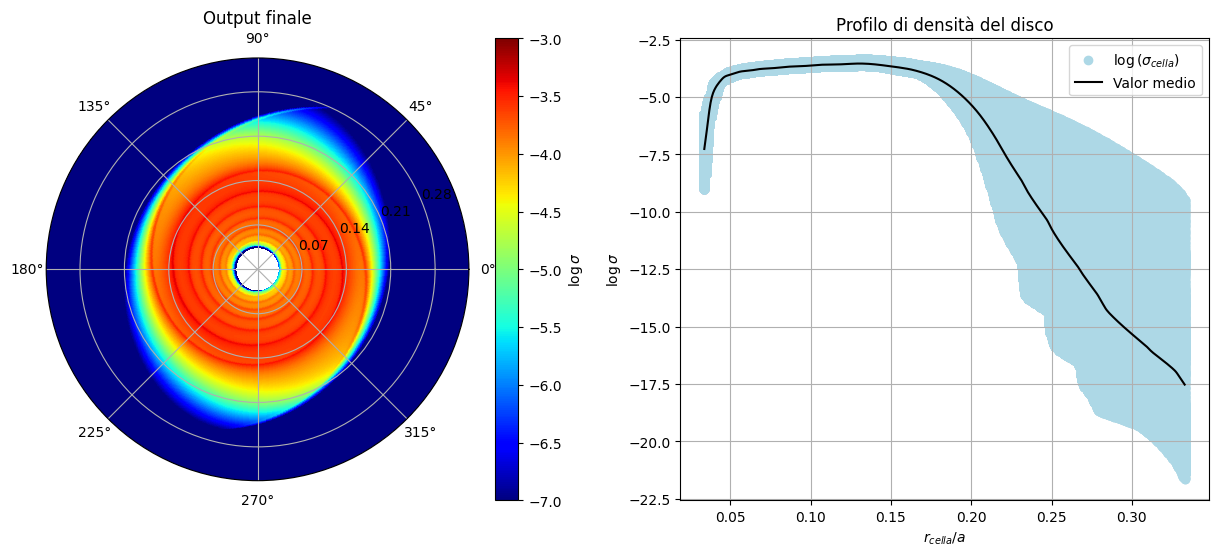
\includegraphics[width=\textwidth]{Immagini/Simulazioni/cal_mass.png}
    \caption{Calcolo della massa per il disco circum-secondario con $q\,=\,0.33$, $e\,=\,0.0$. L'output analizzato è quello alla cinquantesima orbita della binaria. La Figura di destra riporta sovrapposti uno scatter delle masse delle singole celle ed il valor medio della massa per cella nelle varie corone circolari. Notiamo come mediare sulla coordinata azimutale determini la perdita di alcune caratteristiche del disco.}
    \label{fig:mass_grid}
\end{figure}

\textbf{Energia meccanica}\\

L'energia meccanica per le celle viene calcolata come
\begin{equation}
E_{cella}\,=\,\frac{1}{2}m_{cella} \cdot(u_r^2\,+\,u_\theta^2)\,-\frac{m_{cella}}{r_{cella}}
\label{eq:ene_cella}
\end{equation}
dove $E_{cella}$ è l'energia della singola cella ed $r_{cella}$ è la coordinata radiale del centro della cella.
Nella \eqref{eq:ene_cella} $M_\ast$ e $G$ non compaiono poiché sono pari ad uno: il contributo potenziale dovuto al secondo corpo è trascurato poiché stiamo lavorando nella Roche-Lobe del corpo al centro della griglia.
In Figura \ref{fig:ene_grid} è riportato un esempio di calcolo di $E_{cella}$.\\

\textbf{Momento angolare}\\

Il momento angolare della singola cella $L_{cella}$ viene calcolato tenendo conto della sola velocità azimutale come
\begin{equation}
L_{cella}\,=\,m_{cella} \cdot u_\theta \cdot r_{min-cella}
\label{eq:moma_cella}
\end{equation}
dove $r_{min-cella}$ è la coordinata radiale del bordo della cella a raggio minore. Lavorare con $r_{min-cella}$ è necessario poiché la velocità è un campo sfalsato in FARGO3D. In Figura \ref{fig:moma_grid} è riportato un esempio di calcolo di $L_{cella}$.

\begin{figure}[H]
    \centering
    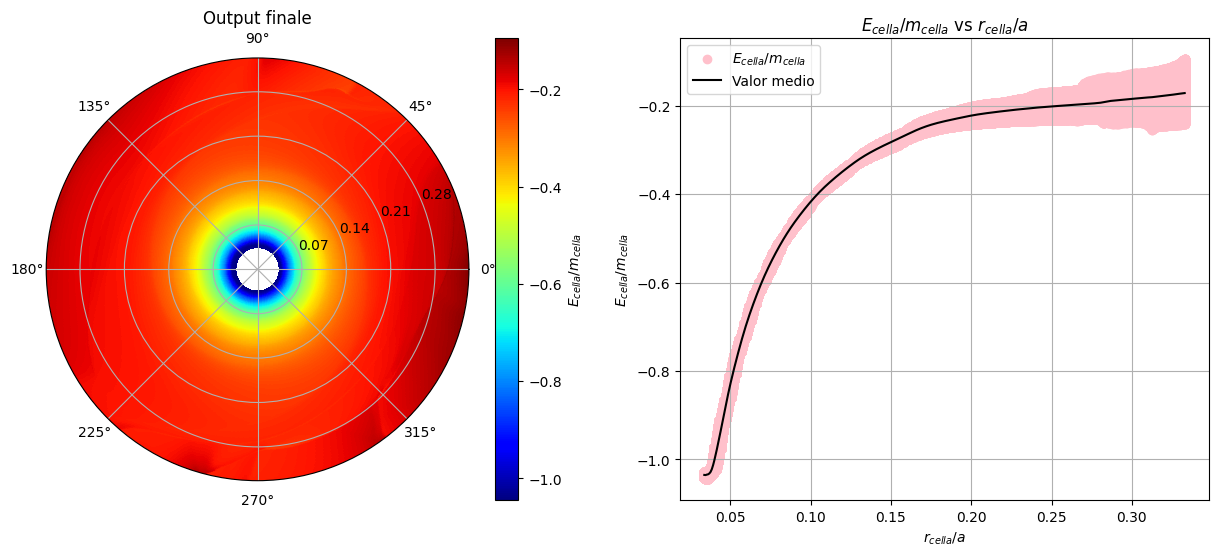
\includegraphics[width=\textwidth]{Immagini/Simulazioni/cal_ene.png}
    \caption{Calcolo dell'energia meccanica per il disco circum-secondario con $q\,=\,0.33$, $e\,=\,0.0$. L'output analizzato è quello alla cinquantesima orbita della binaria. La Figura di destra riporta sovrapposti uno scatter delle energie delle singole celle ed il valor medio dell'energia per cella nelle varie corone circolari. Notiamo che l'energia è minore nella regione in cui è presente il materiale, poiché il gas è gravitazionalmente legato alla stella posta al centro della griglia.}
    \label{fig:ene_grid}
\end{figure}

\begin{figure}[H]
    \centering
    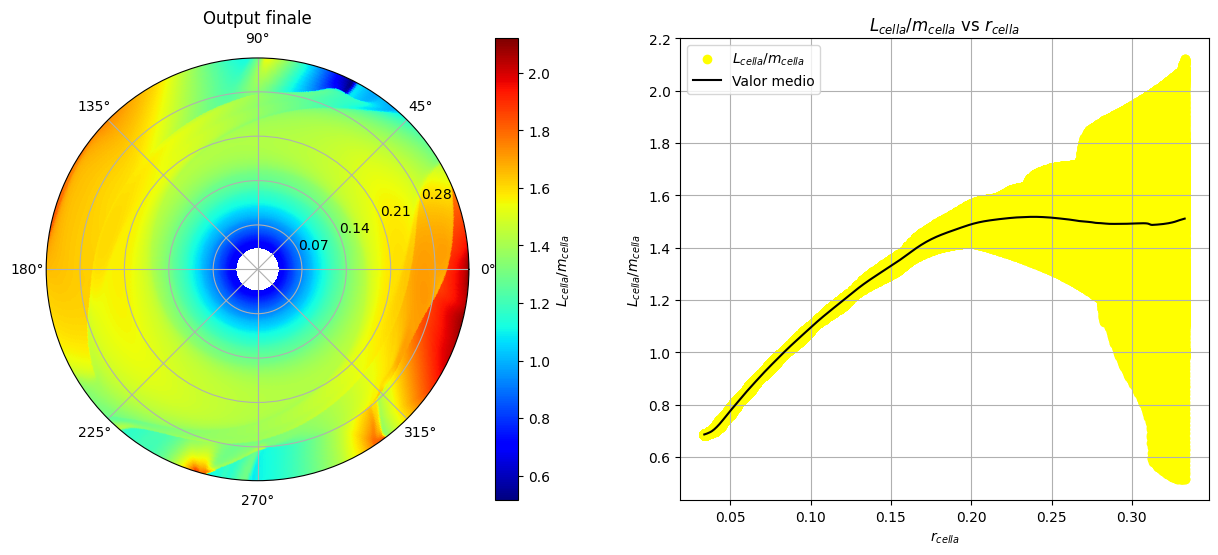
\includegraphics[width=\textwidth]{Immagini/Simulazioni/cal_moma.png}
    \caption{Calcolo del momento angolare per il disco circum-secondario con $q\,=\,0.33$, $e\,=\,0.0$. L'output analizzato è quello alla cinquantesima orbita della binaria. La Figura di destra riporta sovrapposti uno scatter di $L_{cella}$ ed il valor medio di $L_{cella}$ nelle varie corone circolari.}
    \label{fig:moma_grid}
\end{figure}

\newpage

Vogliamo ora determinare dei criteri che ci consentano di determinare le caratteristiche dei dischi. Siamo in particolare interessati alla determinazione delle dimensioni dei dischi e alle loro eccentricità

\subsection{Calcolo del raggio di troncamento}

Dobbiamo fornire un criterio che ci consenta di determinare le dimensioni della regione spaziale occupata dal disco: $r_T$ delimita il cerchio contenente il $99.9 \%$ della massa di gas presente nel dominio simulato. Per calcolare tale raggio lavoriamo con le corone circolari concentriche che costituiscono la griglia. Valutiamo la massa progressiva, ossia la somma di $m_{cella}$ effettuata su tutte quelle celle che hanno posizione centrale per $r\,<\,r_{lim}$, dove $r_{lim}$ è un certo valore limite. Quando nella regione caratterizzata da $r\,<\,r_{lim}$ raggiunge il valore prefissato di massa, abbiamo determinato il raggio di troncamento. In Figura \ref{fig:cal_tr} è riportato un esempio di calcolo del raggio di troncamento.

\begin{figure}[H]
    \centering
    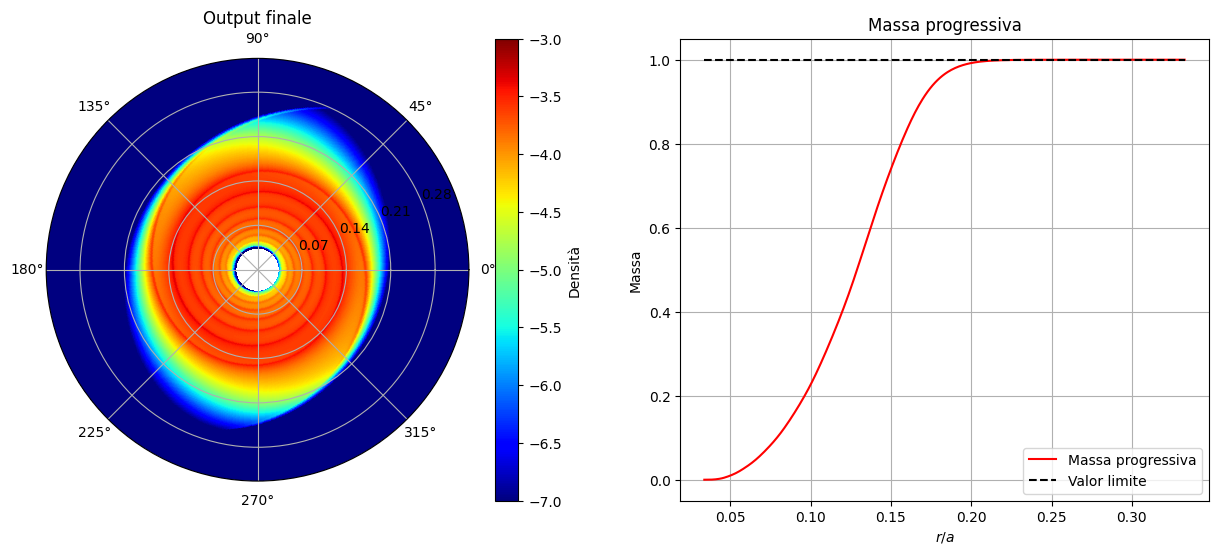
\includegraphics[width=\textwidth]{Immagini/Simulazioni/cal_rt.png}
    \caption{Calcolo del raggio di troncamento per il disco circum-secondario con $q\,=\,0.33$, $e\,=\,0.0$. L'output analizzato è quello alla cinquantesima orbita della binaria. La Figura di destra riporta la massa progressiva ed il valore limite del $99.9\%$ della massa. Per il disco in questione si ha che: $r_T\,=\,0.221\,a$.}
    \label{fig:cal_tr}
\end{figure}

\subsection{Calcolo del semiasse maggiore di troncamento}

Alcuni dischi circumstellari sono eccentrici: procedere con un metodo come quello esposto precedentemente implica commettere degli errori nella determinazione dell'effettiva dimensione del disco. Per ovviare a queste problematiche abbiamo calcolato il semiasse maggiore di troncamento $a_T$ come segue. In primo luogo si calcola il valore del semiasse per ogni cella costituente la griglia. Dato che stiamo lavorando trascurando il contributo all'energia dovuto al corpo perturbante possiamo utilizzare i risultati ottenuti durante l'analisi del problema di Keplero (vedi Sezione \ref{sec:Keplero}). Il semiasse dell'orbita del materiale contenuto nella singola cella è allora:
\begin{equation}
a_{cella}\,=\,-\frac{m_{cella}}{2\cdot E_{cella}}
\label{eq:sax_cella}
\end{equation}
Una volta calcolati tutti gli $a_{cella}$ si valuta la massa progressiva all'aumentare del semiasse $a_{lim}$: quando la regione interna ad $a_{lim}$ contiene il $99.9\%$ del materiale presente nel dominio simulato abbiamo determinato il semiasse maggiore di troncamento.
In Figura \ref{fig:cal_sax} è riportato un esempio di calcolo del semiasse di troncamento

\begin{figure}[H]
    \centering
    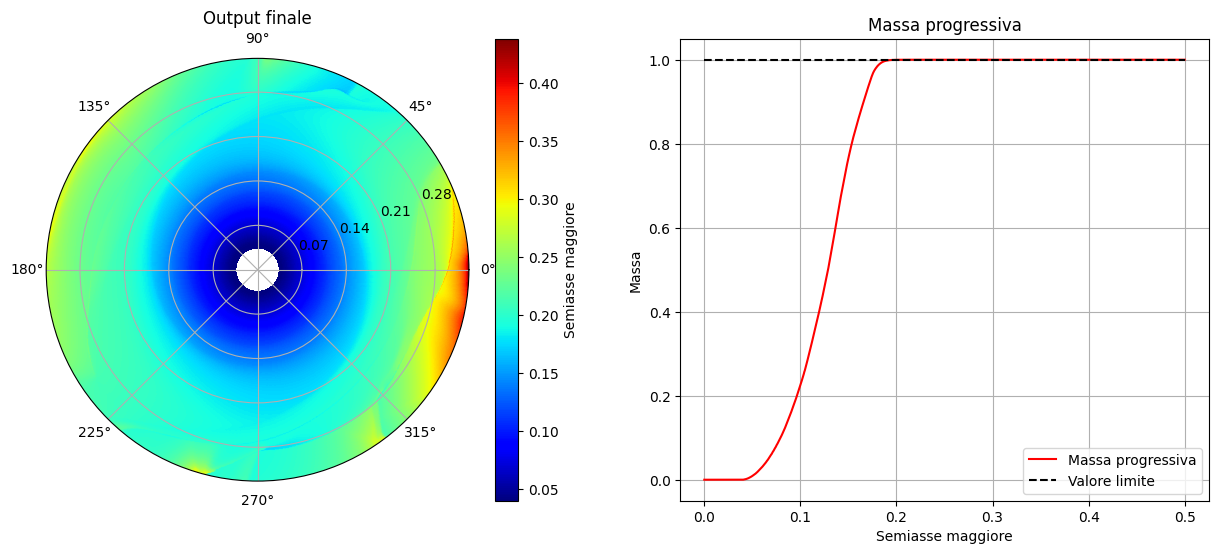
\includegraphics[width=\textwidth]{Immagini/Simulazioni/cal_sax.png}
    \caption{Calcolo del semiasse del disco circum-secondario con $q\,=\,0.33$, $e\,=\,0.0$. L'output analizzato è quello alla cinquantesima orbita della binaria. La figura di sinistra riporta i valori di semiasse assunti dalle varie celle della griglia. La Figura di destra riporta la massa progressiva ed il valore limite del $99.9\%$ della massa. Per il disco in questione si ha che: $a_T\,=\,0.193\,a$.}
    \label{fig:cal_sax}
\end{figure}

\subsection{Calcolo dell'eccentricità del disco}

Un'informazione aggiuntiva sul disco può essere ricavata una volta note l'energia ed il momento angolare in tutta la griglia, come visto in Sezione \ref{sec:Keplero}. L'eccentricità dell'orbita del materiale contenuto nelle varie celle viene ricavata come
\begin{equation}
e_{cella}\,=\,\sqrt{1\,-\,\frac{(r_{cella}\cdot u_\theta)^2}{a_{cella}}},
\label{eq:ecc_cella}
\end{equation}
dove abbiamo approssimato $m_{cella}$ a zero poiché $m_{cella} \ll 1$.
Per determinare l'eccentricità del disco $e_{disco}$ valutiamo quale sia il valor medio di $e_{cella}$ nell'intorno si $a_T$, ossia considerando solamente quelle celle che hanno $a_{cella}$ confrontabile con il semiasse maggiore del disco. In Figura \ref{fig:cal_ecc} è riportato un esempio di calcolo del semiasse di troncamento

\begin{figure}[H]
    \centering
    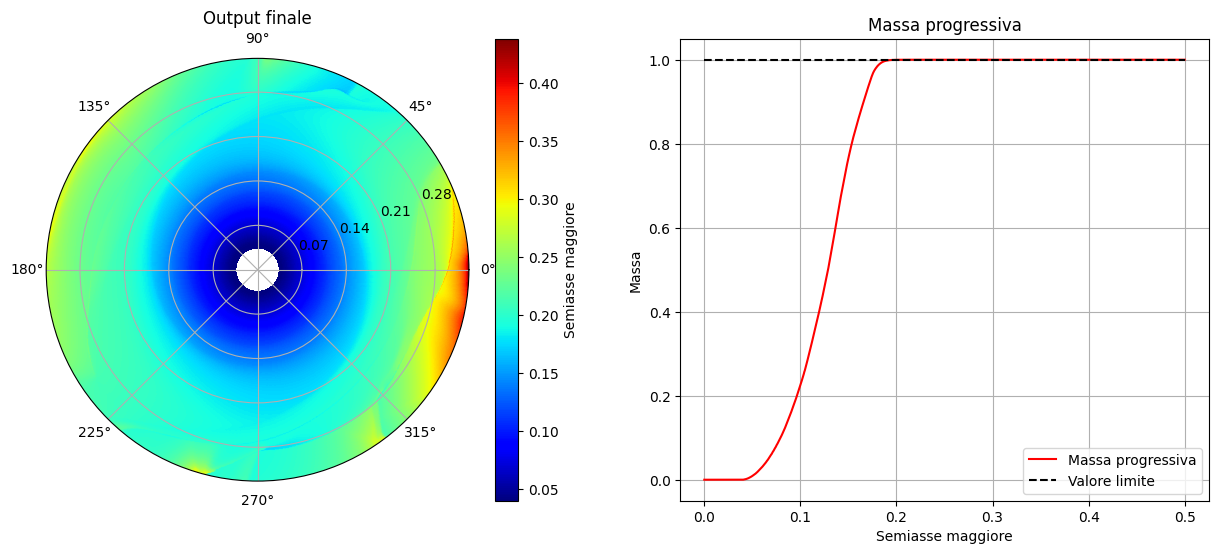
\includegraphics[width=\textwidth]{Immagini/Simulazioni/cal_sax.png}
    \caption{Calcolo dell'eccentricità del disco circum-secondario con $q\,=\,0.33$, $e\,=\,0.0$. L'output analizzato è quello alla cinquantesima orbita della binaria. La figura di sinistra riporta i valori di eccentricità assunti nelle varie celle della griglia. La Figura di destra riporta il profilo d'eccentricità del disco.}
    \label{fig:cal_sax}
\end{figure}